% Flow diagram of the demand model (noga/model.py @ d79d200+dirty).
% Regenerate with the /draw-model command.
\documentclass[tikz,border=8pt]{standalone}
\usepackage[T1]{fontenc}
\usepackage{lmodern}
\usepackage{amsmath}
\usetikzlibrary{positioning,fit,arrows.meta,calc,backgrounds}

% One colour per role (light fill, darker border).
\definecolor{inF}{HTML}{E3F0FB}\definecolor{inD}{HTML}{2F6FA8}
\definecolor{prF}{HTML}{EAF6EA}\definecolor{prD}{HTML}{3C8A3C}
\definecolor{trF}{HTML}{F1ECF8}\definecolor{trD}{HTML}{6A4C9C}
\definecolor{dhF}{HTML}{FDF0E1}\definecolor{dhD}{HTML}{C0711B}
\definecolor{phF}{HTML}{FBE8EC}\definecolor{phD}{HTML}{B03A55}
\definecolor{tnF}{HTML}{F2F2F2}\definecolor{tnD}{HTML}{6B6B6B}

\tikzset{
  box/.style={draw, rounded corners=3pt, line width=0.8pt, align=center,
    inner sep=4pt, minimum height=11mm, font=\small},
  inp/.style={box, fill=inF, draw=inD},
  pre/.style={box, fill=prF, draw=prD},
  tr/.style={box, fill=trF, draw=trD},
  dh/.style={box, fill=dhF, draw=dhD},
  ph/.style={box, fill=phF, draw=phD},
  tn/.style={box, fill=tnF, draw=tnD, align=left, minimum height=0pt},
  arr/.style={-{Stealth[length=2.4mm]}, line width=0.8pt, draw=black!70},
  raw/.style={arr, draw=inD, line width=1.1pt},
  w/.style={font=\scriptsize, fill=white, inner sep=1.2pt},
  swatch/.style={minimum height=3mm, minimum width=5mm, inner sep=0pt},
}
\newcommand{\T}[2]{\textbf{#1}\\[-1pt]{\footnotesize #2}}

\begin{document}
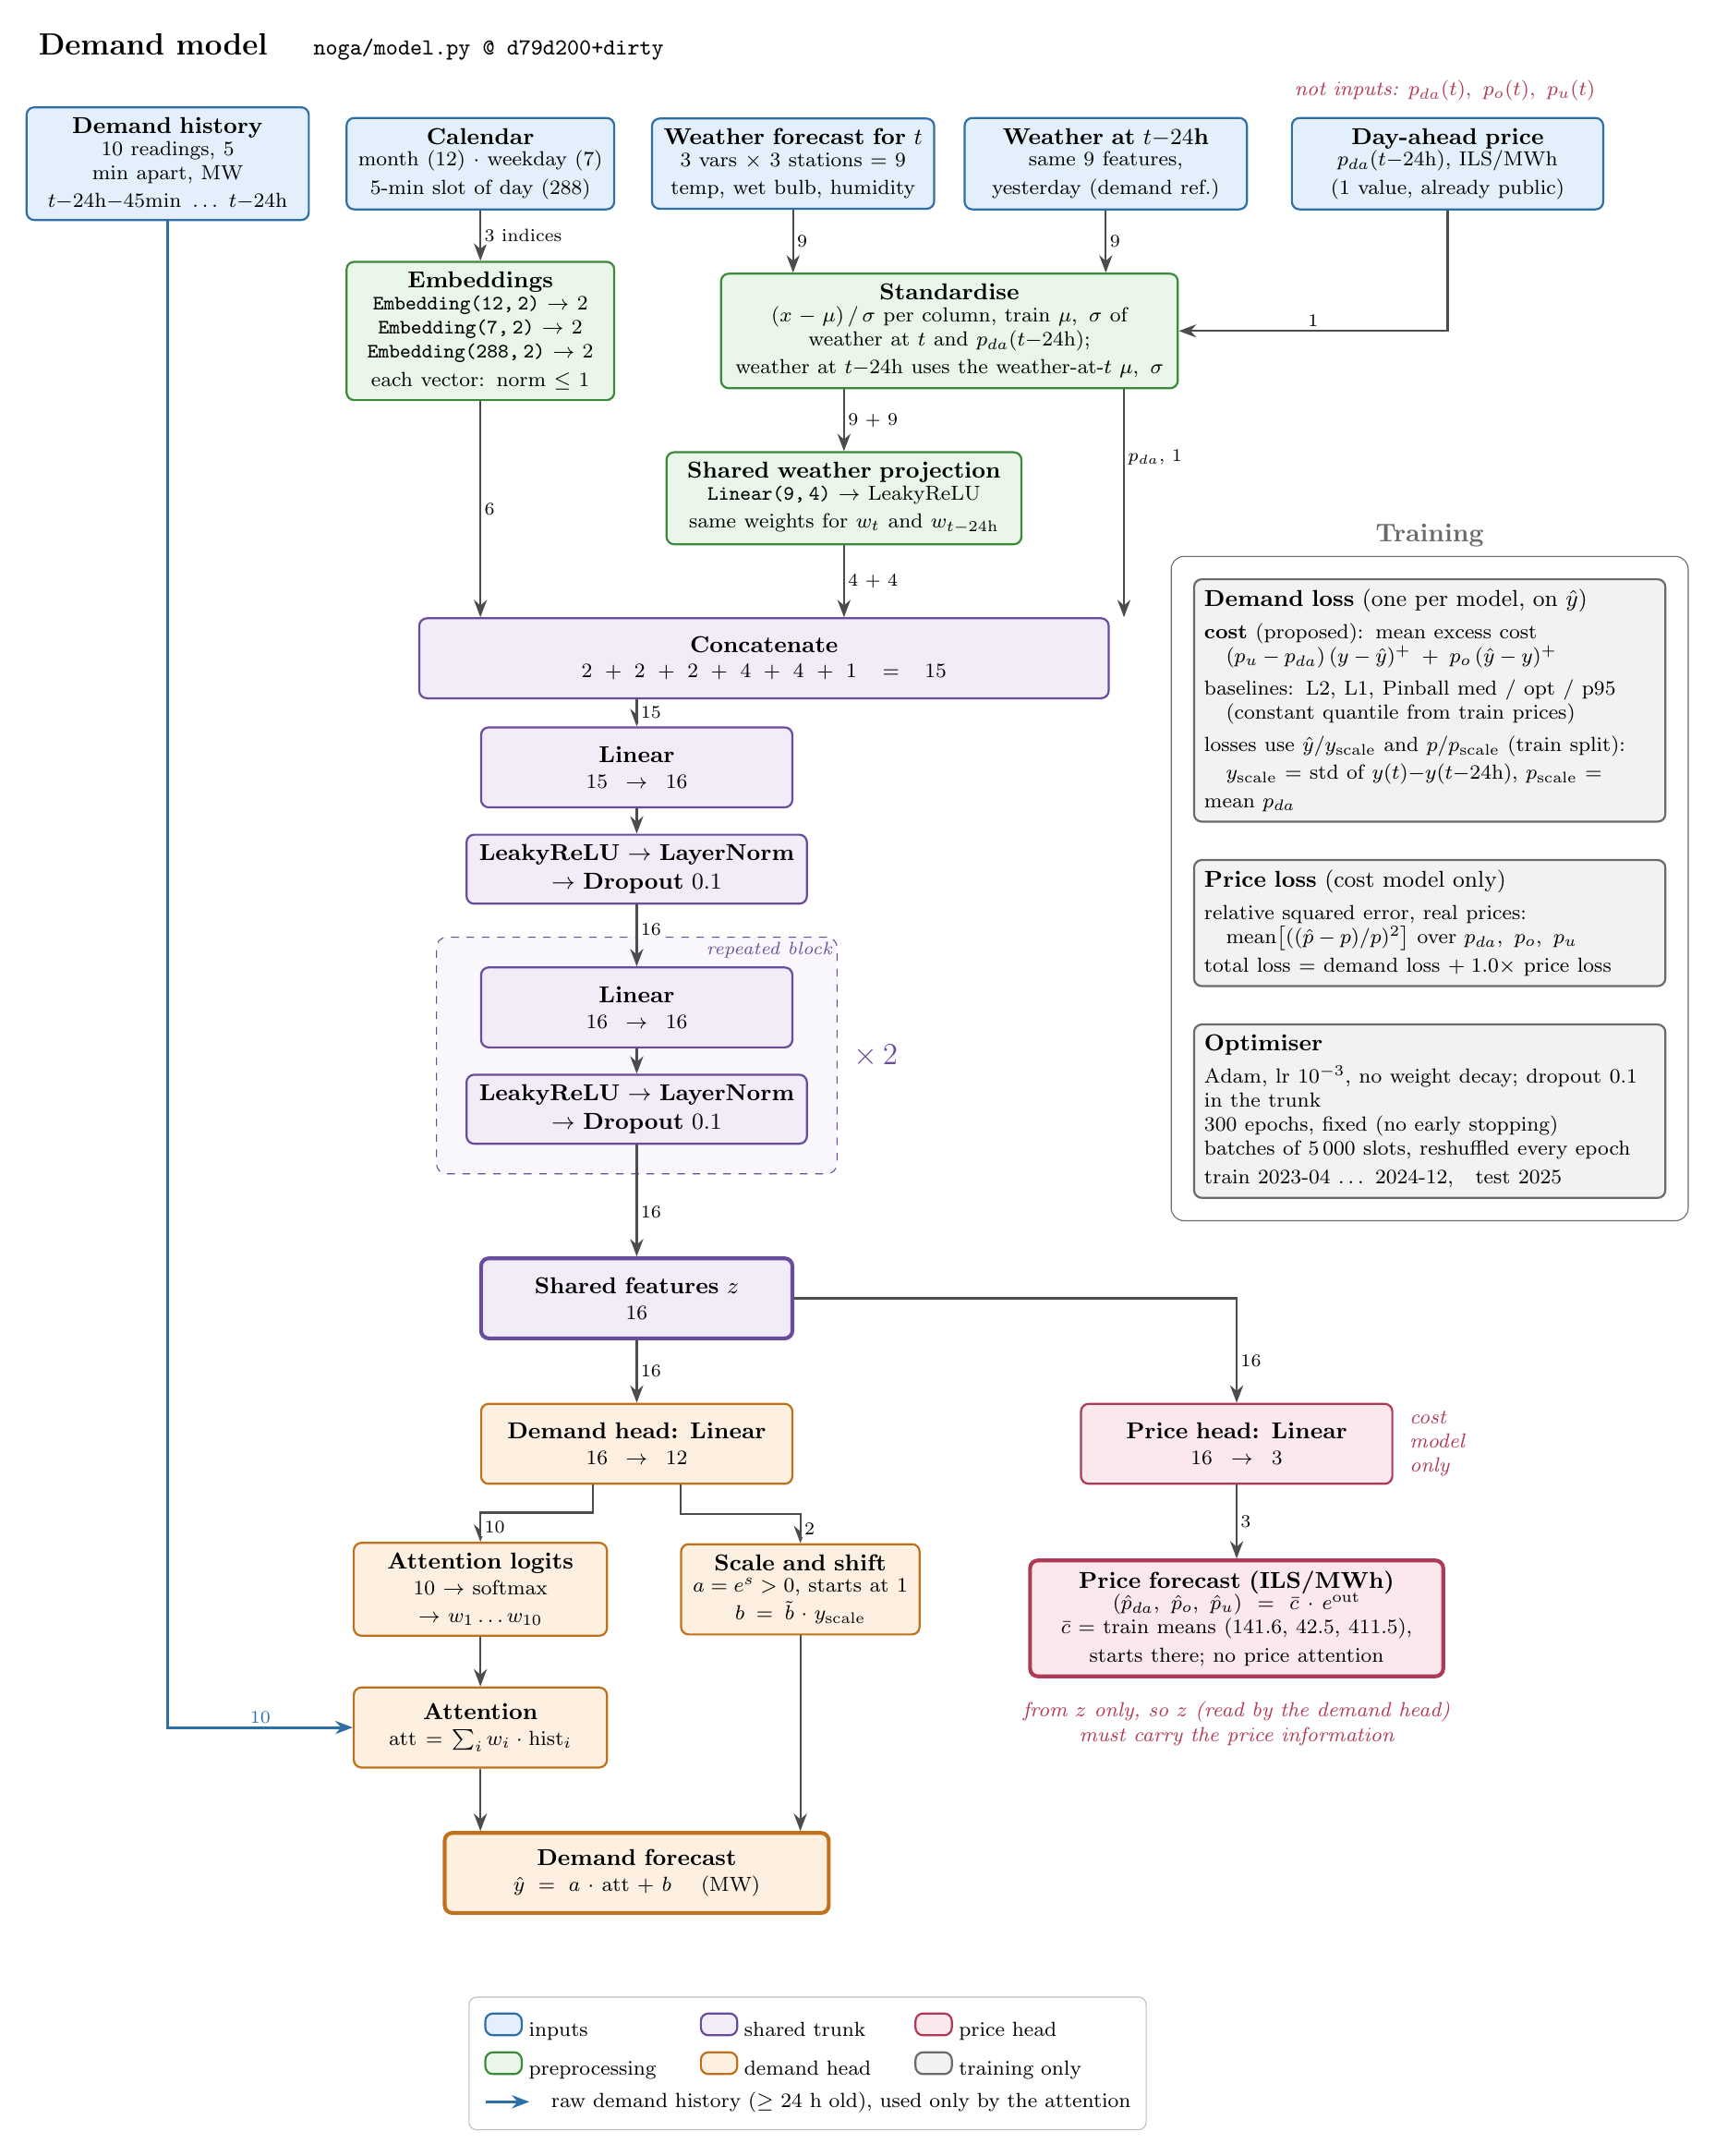
\begin{tikzpicture}

% ---------------------------------------------------------------- title
\node[font=\large\bfseries, anchor=west] (title) at (-6.2, 1.6)
  {Demand model \quad{\normalfont\ttfamily\small noga/model.py @ d79d200+dirty}};

% ---------------------------------------------------------------- inputs
\node[inp, text width=36mm] (hist) at (-4.3, 0)
  {\T{Demand history}{10 readings, 5 min apart, MW\\$t{-}24\text{h}{-}45\text{min}\;\ldots\;t{-}24\text{h}$}};
\node[inp, text width=34mm] (cal) at (0, 0)
  {\T{Calendar}{month (12) $\cdot$ weekday (7)\\5-min slot of day (288)}};
\node[inp, text width=36mm] (wx) at (4.3, 0)
  {\T{Weather forecast for $t$}{3 vars $\times$ 3 stations $=$ 9\\temp, wet bulb, humidity}};
\node[inp, text width=36mm] (wxp) at (8.6, 0)
  {\T{Weather at $t{-}24\text{h}$}{same 9 features,\\yesterday (demand ref.)}};
\node[inp, text width=40mm] (ph) at (13.3, 0)
  {\T{Day-ahead price}{$p_{da}(t{-}24\text{h})$, ILS/MWh\\(1 value, already public)}};
\node[font=\footnotesize\itshape, text=phD, anchor=south east]
  at ($(ph.north east)+(0,1mm)$) {not inputs: $p_{da}(t),\ p_o(t),\ p_u(t)$};

% ---------------------------------------------------------------- preprocessing
\node[pre, text width=34mm] (emb) at (0, -2.3)
  {\T{Embeddings}{\texttt{Embedding(12,\,2)} $\to$ 2\\\texttt{Embedding(7,\,2)} $\to$ 2\\\texttt{Embedding(288,\,2)} $\to$ 2\\each vector: norm $\leq 1$}};
\node[pre, text width=60mm] (scale) at (6.45, -2.3)
  {\T{Standardise}{$(x - \mu) \,/\, \sigma$ per column, train $\mu,\ \sigma$ of\\weather at $t$ and $p_{da}(t{-}24\text{h})$;\\weather at $t{-}24\text{h}$ uses the weather-at-$t$ $\mu,\ \sigma$}};
\node[pre, text width=46mm] (proj) at (5.0, -4.6)
  {\T{Shared weather projection}{\texttt{Linear(9,\,4)} $\to$ LeakyReLU\\same weights for $w_t$ and $w_{t-24\text{h}}$}};

\draw[arr] (cal) -- node[w,right]{3 indices} (emb);
\draw[arr] (wx) -- node[w,right]{9} (wx |- scale.north);
\draw[arr] (wxp) -- node[w,right]{9} (wxp |- scale.north);
\draw[arr] (ph.south) |- node[w,pos=0.75,above]{1} (scale.east);
\draw[arr] (proj.north |- scale.south) -- node[w,right]{9 + 9} (proj.north);

% ---------------------------------------------------------------- concat
\node[tr, text width=92mm] (cat) at (3.9, -6.8)
  {\T{Concatenate}{$2 + 2 + 2 + 4 + 4 + 1 = 15$}};
\draw[arr] (emb.south) -- node[w,right]{6} (emb.south |- cat.north);
\draw[arr] (proj.south) -- node[w,right]{4 + 4} (proj.south |- cat.north);
\coordinate (pda) at ($(scale.south)+(24mm,0)$);
\draw[arr] (pda) -- node[w,right,pos=0.3]{$p_{da}$, 1} (pda |- cat.north);

% ---------------------------------------------------------------- trunk
\node[tr, text width=40mm] (l0) at (2.15, -8.3) {\T{Linear}{$15 \to 16$}};
\node[tr, text width=44mm, minimum height=8mm] (a0) at (2.15, -9.7)
  {\textbf{LeakyReLU} $\to$ \textbf{LayerNorm}\\$\to$ \textbf{Dropout} 0.1};
\node[tr, text width=40mm] (l1) at (2.15, -11.6) {\T{Linear}{$16 \to 16$}};
\node[tr, text width=44mm, minimum height=8mm] (a1) at (2.15, -13.0)
  {\textbf{LeakyReLU} $\to$ \textbf{LayerNorm}\\$\to$ \textbf{Dropout} 0.1};
\begin{scope}[on background layer]
  \node[draw=trD, dashed, rounded corners=4pt, fill=trF!40,
        fit=(l1)(a1), inner sep=4mm] (blk) {};
\end{scope}
\node[font=\bfseries\large, text=trD, anchor=west] at ($(blk.east)+(1mm,0)$) {$\times\,2$};
\node[font=\scriptsize\itshape, text=trD, anchor=north east, inner sep=2pt]
  at (blk.north east) {repeated block};
\node[tr, text width=40mm, line width=1.5pt] (z) at (2.15, -15.6)
  {\T{Shared features $z$}{16}};

\draw[arr] (cat.south -| l0) -- node[w,right]{15} (l0);
\draw[arr] (l0) -- (a0);
\draw[arr] (a0) -- node[w,right,pos=0.4]{16} (l1);
\draw[arr] (l1) -- (a1);
\draw[arr] (a1) -- node[w,right,pos=0.6]{16} (z);

% ---------------------------------------------------------------- demand head
\node[dh, text width=40mm] (dl) at (2.15, -17.6) {\T{Demand head: Linear}{$16 \to 12$}};
\node[dh, text width=32mm] (logit) at (0, -19.6)
  {\T{Attention logits}{10 $\to$ softmax $\to$ $w_1 \ldots w_{10}$}};
\node[dh, text width=30mm] (ab) at (4.4, -19.6)
  {\T{Scale and shift}{$a = e^{s} > 0$, starts at 1\\$b = \tilde b \cdot y_{\text{scale}}$}};
\node[dh, text width=32mm] (att) at (0, -21.5)
  {\T{Attention}{$\text{att} = \sum_i w_i \cdot \text{hist}_i$}};
\node[dh, line width=1.5pt, text width=50mm] (yhat) at (2.15, -23.5)
  {\T{Demand forecast}{$\hat y = a \cdot \text{att} + b$ \quad (MW)}};

\draw[arr] (z) -- node[w,right]{16} (dl);
\draw[arr] ($(dl.south)+(-6mm,0)$) |- ($(logit.north)+(0,4mm)$) -- node[w,right]{10} (logit.north);
\draw[arr] ($(dl.south)+(6mm,0)$)  |- ($(ab.north)+(0,4mm)$) -- node[w,right]{2} (ab.north);
\draw[arr] (logit) -- (att);
\draw[arr] (att.south) -- (att.south |- yhat.north);
\draw[arr] (ab.south) -- (ab.south |- yhat.north);
\draw[raw] (hist.south) -- (hist.south |- att) -- node[w,above,text=inD]{10} (att.west);

% ---------------------------------------------------------------- price head
\node[ph, text width=40mm] (pl) at (10.4, -17.6) {\T{Price head: Linear}{$16 \to 3$}};
\node[font=\footnotesize\itshape, text=phD, anchor=west, align=left] at ($(pl.east)+(1mm,0)$)
  {cost\\model\\only};
\node[ph, line width=1.5pt, text width=54mm] (pout) at (10.4, -20.0)
  {\T{Price forecast (ILS/MWh)}{$(\hat p_{da},\ \hat p_o,\ \hat p_u) = \bar c \cdot e^{\text{out}}$\\
   $\bar c$ = train means (141.6, 42.5, 411.5),\\starts there; no price attention}};
\node[font=\footnotesize\itshape, text=phD, align=center, anchor=north] at ($(pout.south)+(0,-2mm)$)
  {from $z$ only, so $z$ (read by the demand head)\\must carry the price information};

\draw[arr] (z.east) -| node[w,pos=0.8,right]{16} (pl.north);
\draw[arr] (pl) -- node[w,right]{3} (pout);

% ---------------------------------------------------------------- training panel
\node[tn, text width=62mm, anchor=north west] (loss) at (9.8, -5.7)
  {\textbf{Demand loss} (one per model, on $\hat y$)\\[3pt]
   \footnotesize
   \textbf{cost} (proposed): mean excess cost\\
   \quad $(p_u - p_{da})\,(y-\hat y)^+ \;+\; p_o\,(\hat y - y)^+$\\[3pt]
   baselines: L2, L1, Pinball med / opt / p95\\
   \quad (constant quantile from train prices)\\[3pt]
   losses use $\hat y / y_{\text{scale}}$ and $p / p_{\text{scale}}$ (train split):\\
   \quad $y_{\text{scale}}$ = std of $y(t){-}y(t{-}24\text{h})$, $p_{\text{scale}}$ = mean $p_{da}$};
\node[tn, text width=62mm, anchor=north west] (ploss) at ($(loss.south west)+(0,-5mm)$)
  {\textbf{Price loss} (cost model only)\\[3pt]
   \footnotesize
   relative squared error, real prices:\\
   \quad $\text{mean}\big[((\hat p - p)/p)^2\big]$ over $p_{da},\ p_o,\ p_u$\\
   total loss $=$ demand loss $+\; 1.0 \times$ price loss};
\node[tn, text width=62mm, anchor=north west] (opt) at ($(ploss.south west)+(0,-5mm)$)
  {\textbf{Optimiser}\\[3pt]
   \footnotesize
   Adam, lr $10^{-3}$, no weight decay; dropout 0.1 in the trunk\\
   300 epochs, fixed (no early stopping)\\
   batches of 5\,000 slots, reshuffled every epoch\\
   train 2023-04 \ldots\ 2024-12, \; test 2025};
\begin{scope}[on background layer]
  \node[draw=tnD, rounded corners=5pt, fill=white, fit=(loss)(ploss)(opt),
        inner sep=3mm, label={[font=\bfseries, text=tnD]north:Training}] (trainp) {};
\end{scope}

% ---------------------------------------------------------------- legend
\node[anchor=north, font=\footnotesize, draw=black!25, rounded corners=3pt,
      inner sep=6pt] (leg) at (4.5, -25.2)
  {\begin{tabular}{@{}l@{\;}l@{\qquad}l@{\;}l@{\qquad}l@{\;}l@{}}
   \tikz\node[inp,swatch]{}; & inputs &
   \tikz\node[tr,swatch]{}; & shared trunk &
   \tikz\node[ph,swatch]{}; & price head\\[3pt]
   \tikz\node[pre,swatch]{}; & preprocessing &
   \tikz\node[dh,swatch]{}; & demand head &
   \tikz\node[tn,swatch]{}; & training only\\[3pt]
   \multicolumn{6}{@{}l@{}}{\tikz[baseline=-0.6ex]\draw[raw](0,0)--(6mm,0);
     \; raw demand history ($\geq$ 24 h old), used only by the attention}
   \end{tabular}};

\end{tikzpicture}
\end{document}
